% Created 2011-07-10 dom 13:39
\documentclass[12pt]{article}
\usepackage[utf8]{inputenc}
\usepackage[T1]{fontenc}
\usepackage{fixltx2e}
\usepackage{graphicx}
\usepackage{longtable}
\usepackage{float}
\usepackage{wrapfig}
\usepackage{soul}
\usepackage{textcomp}
\usepackage{marvosym}
\usepackage{xspace}
\usepackage{latexsym}
\usepackage{amssymb}
\usepackage[usenames,dvipsnames,svgnames,table]{xcolor}
\usepackage{hyperref}
\definecolor{darkblue}{rgb}{0.0,0.1,0.3}
\definecolor{darkgreen}{rgb}{0.0,0.35,0.15}
\definecolor{darkred}{rgb}{0.3,0.1,0.0}
\def\refColor{darkgreen}
\hypersetup{%
  colorlinks,
  linkcolor=\refColor,
  urlcolor=\refColor,
  anchorcolor=\refColor,
  citecolor=\refColor
}
\usepackage[hmargin={2.5cm,2cm}]{geometry}
\tolerance=1000
\usepackage{listings}
\usepackage{math,ff++listings}
\usepackage{pgf}

\usepackage[noblocks]{authblk} % Authors
\setlength{\affilsep}{3em}

\providecommand{\alert}[1]{\textbf{#1}}
\providecommand{\structure}[1]{#1}

\newcommand{\FF}{\textit{FreeFem++}\xspace}
\newcommand{\FFcs}{\textit{FreeFem-cs}\xspace}
\renewcommand{\P}{\mathcal{P}_}
\newcommand{\R}{{\mathbb R}}

\newcounter{exercise}
\newenvironment{exercise}{%
  \stepcounter{exercise}
  \subsubsection*{Exercise~\theexercise.}}
{}

\title{Computer Practices: The Finite Element Method with \FF}

\author[$\dagger$]{Juan Vicente Gutiérrez Santacreu}
\author[$\ddagger$]{J. Rafael Rodríguez Galván}
\affil[$\dagger$]{Departamento de Matemática Aplicada I. Universidad de Sevilla. \texttt{juanvi@us.es}}
\affil[$\ddagger$]{Departamento de Matemáticas. Universidad de Cádiz. \texttt{rafael.rodriguez@uca.es}}

\date{
  \textsf{\textit{Doc-Course: ``Partial Differential Equations:
      Analysis, Numerics and Control''. Research Unit 3: Numerical
      Methods for PDEs}}
  \\[2em]
  \emph{April, 2018}
  \\[10em]
  
\includegraphics[width=0.07\textwidth]{./cc-by-sa.png}
  \\[1em]
  \begin{small} \scriptsize\em
    \href{http://creativecommons.org/licenses/by-sa/3.0/}{Creative
      Commons Attribution-Share\_Alike License, \\
      \scriptsize\url{http://creativecommons.org/licenses/by-sa/3.0/}}.
  \end{small}
}

% -----------------------------------
% Code listing style
% -----------------------------------
\definecolor{codegreen}{rgb}{0,0.6,0}
\definecolor{codegray}{rgb}{0.5,0.5,0.5}
\definecolor{codepurple}{rgb}{0.58,0,0.82}
\definecolor{backcolour}{rgb}{0.94,0.94,0.95}

\lstdefinestyle{mystyle}{
    % backgroundcolor=\color{backcolour},
    % commentstyle=\color{codegreen},
    % keywordstyle=\color{magenta},
    % numberstyle=\tiny\color{codegray},
    % stringstyle=\color{codepurple},
    % % basicstyle=\footnotesize,
    % breakatwhitespace=false,
    % breaklines=true,
    % numbers=left,
    % numbersep=5pt,
}
\lstset{style=mystyle}
% -----------------------------------


% -----------------------------------
\begin{document}
% -----------------------------------

\maketitle

%\large %%%%%%%%%%%%%%%%%%%%%%%%%%%%%%%%

\newpage
\setcounter{tocdepth}{2}
\tableofcontents
\vspace*{1cm}

\section{Introduction}
\label{sec:introduction}

\subsection{The \FF environment}
\label{sec:ff-environment}

\alert{\FF}\footnote{\url{http://www.freefem.org/ff++}} is a package
for \emph{numerical approximation of the solution of PDE} (partial
differential equations), both 2D and 3D, by means of the \textit{Finite
Element Method} (FEM). \FF is composed of:

\begin{itemize}

\item An interpreted \alert{programming Language}:
  \begin{itemize}
  \item Oriented to (1) fast specification of (linear and steady) PDE
    problems and (2) resolution of those problems, using the FEM.
  \item Allows easy implementation of complex problems (nonlinear,
    transient,...)
  \end{itemize}

\item An \alert{interpreter} for that language.
  \begin{itemize}

  \item Programs in FreeFem++ are interpreted (not compiled) at
    runtime. In this sense, FreeFem++ is a \textit{scripting} language
    (like Python, Matlab/Octave, Perl, and others).
  \item \FF is \alert{open source}/\alert{free software} (GNU GPL license).
  \item There are different versions: \texttt{FreFem++},
    \texttt{FreeFem++-nw}, \texttt{FreeFem++-mpi},\ldots{}
  \end{itemize} % ends low level
\end{itemize} % ends low level

\FF is mainly developed by \textbf{F. Hetch}.
\begin{center}
  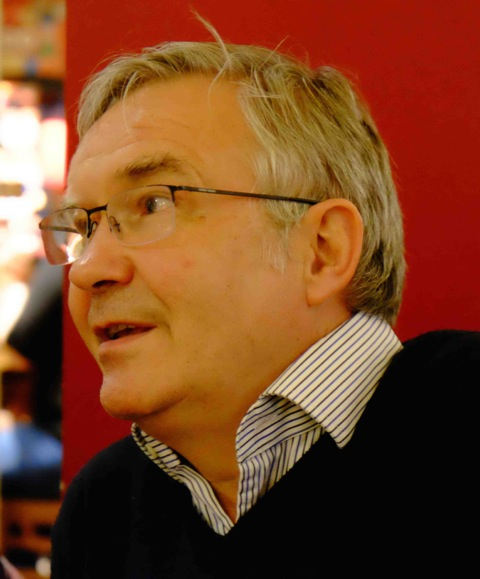
\includegraphics[width=0.3\linewidth]{./Hecht-portrait}
\end{center}

\subsection{What can you do with \FF?}
Some examples related to 2D steady Stokes equations:
\begin{equation*}
  \left\{
  \begin{aligned}
    -\nu\Delta \mathbf{u}+ \nabla p &= f
    \\
    \nabla\cdot \mathbf{u} & = 0
    \\ & + \text{boundary conditions},
  \end{aligned}
  \right.
\end{equation*}
where the unknowns are $\mathbf{u}=(u,v):\Omega\to\R^2$ (velocity field of fluid)
and $p:\Omega\to\R$ pressure in each point of the domain.
\begin{itemize}
\item
  \href{https://www.youtube.com/watch?v=dn4UeMQDf9c&index=2&list=UUbv6VZ2UBw4iXCMR2L4G0zg&t=0s}{Video:
    Stokes/Navier-Stokes equations in Mediterranean sea.}
\item Why I like numerical simulation (as mathematician): it helps you
  to understand underlying maths
  (\href{https://www.youtube.com/watch?v=6x8KseewSrU&feature=youtu.be}{Video:
    instability of a numerical scheme}).
\end{itemize}


\subsection{Characteristics  of the \FF Language}
\begin{itemize}

\item Inspired by \alert{C/C++}.
  \begin{itemize}
  \item \emph{Similarities}: Syntax, strong typing\ldots{}
  \item \emph{Does not include}: Pointers, object orienting, \ldots{}
  \end{itemize}

\item \alert{Oriented} to numerical simulation using the finite element method.
  \alert{Capabilities}:
  \begin{itemize}
  \item Definition of the \textbf{geometry} of a problem and 2D/3D meshing.
    Although \FF is not a CAD/CAE environment and then, for complex
    geometries, it is necessary to use external tools.
  \item Variety of available \alert{finite elements}:
    $P_k$--Lagrange, $P_1$--bubble, $P_1$ discontinuous,
    Raviart-Thomas\ldots{}
  \item Flexibility for definition of problems which can be formulated
    in terms of PDE (and expressed by a \alert{variational formulation})
  \item Automation of the task of \textbf{assembling FEM matrices} (involved in
    underlying FEM linear systems) so that this task is \textit{transparent to the
    user}.
  \item Several algorithms for \alert{resolution of those linear
      systems}: LU, Cholesky, Crout, CG, GMRES, UMFPACK\ldots{}
  \item Facilities for \alert{post-processing} and \alert{2D/3D
      visualization}.  Although \FF no is not specialized in
    scientific visualization, it can be complemented with external
    tools for high-quality graphics.
  \item Other issues:
    \begin{itemize}
    \item Excellent documentation (with a plenty of examples and
      tutorials):
      \url{http://www.freefem.org/ff++/ftp/freefem++doc.pdf}.
    \item (Matlab/Octave/Python/Fortran)--like matrix manipulation.
    \item Automatic interpolation between meshes, adaptive refinement,...
    \item Parallel (with MPI) version available
      (\texttt{FreeFem++-mpi}).
    \end{itemize}
  \end{itemize}

\end{itemize} % ends low level

\section{Installation and first steps}
\label{sec:inst-first-steps}

The \FF package includes an interpreter for execution of code but no
editor or integrated environment (with editor, error feedback, syntax
highlighting, etc.) is included. User is allowed to choose his/her
preferred editor between different possibilities, for instance (see
\FF manual for details):

\begin{itemize}
\item \textit{Crimson Editor} or \textit{Notepad++} on Windows,
\item \textit{Fraise editor} on MacOS.
\item \texttt{Emacs} on GNU/Linux, MacOS or Windows. Note that Emacs
  is a free/libre general-purpose (not only specialized in \FF)
  and powerful text editor.
\item \texttt{\FFcs} on GNU/Linux, MacOS or Windows. Note that \FFcs
  is integrated environment specialized in editing and post-processing
  \FF scripts.
\end{itemize}



% Anyway, for a first approach to \FF, we recommend \FFcs,
% \url{http://www.ann.jussieu.fr/~lehyaric/ffcs/}. \FFcs is an
% integrated environment providing \FF, and adequate editor and other
% characteristics. Of course, advanced users may prefer other options.

Here we review the configuration of the last two ones.

\subsection{Using \FF under Emacs}

Emacs can be installed form its
\href{https://www.gnu.org/software/emacs}{web page} of from the
software center of your operative system.

For a \textbf{easy configuration} from scratch, it suffices to
download and unzip \textit{in your home user directory} the file
\texttt{freefem-emacs-basic-config.zip} which can be found in
\url{https://github.com/rrgalvan/freefem-mode/releases}.

For advanced configuration of \FF mode on Emacs, follow the
instructions from \url{https://github.com/rrgalvan/freefem-mode}.



\subsection{\FFcs: an integrated environment for \FF}
\label{sec:freefem-CS}

\FFcs (\textit{CS} $\leftarrow$ Client/Server) is package which contains
both \FF and an integrated environment for \FF providing an intuitive
interface. It adds to \FF the following goodies:
\begin{itemize}
\item Integrated interface, aimed at making users comfortable.
\item Color-coded editor.
\item Automatic highlighting of \FF.
\item Compilation errors, linked back to the EDP source code.
\item Integrated graphics area for 2d and 3d.
\item Online help including documentation in HTML.
\item Multi-platform (Windows--GNU/Linux--MacOS).
\end{itemize}


\subsubsection{Installation}
For installation, you can get your preferred version from
the ``\textit{Download}'' link
(\url{http://www.ann.jussieu.fr/~lehyaric/ffcs/install.php}) and
follow the specific instructions for each  platform (which consist in
only a few steps). For instance:

\begin{itemize}
\item \textit{Windows}: Execute the installation program and follow
  usual steps. Once installed, click on the \textit{FreeFem++-cs} icon
  and start using the application.
\item \textit{GNU/Linux} (\textit{Ubuntu}, \textit{Debian} and
  others): Decompress the \texttt{.tgz} in your preferred location (for
  instance, in the desktop). Run the program \textit{FreeFem++-cs}
  (located in the folder created when decompress).
\item \textit{MacOS}: Decompress the \texttt{.zip} file in your
  preferred location (e.g. in the desktop). Run \textit{FreeFem++cs}.
\end{itemize}

\begin{exercise}
  Download \FFcs from the web (choose the adequate version for your
  preferred operative system) and install it.
\end{exercise}

\begin{exercise}
  Open the FreeFem++ manual,
  \url{http://www.freefem.org/ff++/ftp/freefem++doc.pdf}, and search
  for recommended editors (in Section 1.1). Choose an editor, install
  and configure it for use with \FF.
\end{exercise}

\subsubsection{First steps with \FFcs}

\FFcs is composed of three different panels:
\begin{enumerate}
\item Editor with syntax highlighting (left).
\item Messages returned by the interpreter (bottom).
\item Graphics generated by our numerical simulation (right).
end{enumerate}
\end{enumerate}

Other Characteristics:

\begin{itemize}
\item The FreeFem++ script (program) can be run at any time by
  clicking in the \texttt{Run} buttom (top left), or pressing
  \texttt{Ctrl+Shift+R}.
\item The script can be stopped at any time by clicking the
  \texttt{Kill} button (top left).
\item Dragging a \FF script file into \FFcs (icon or editor) makes \FFcs
  edit that script.
\end{itemize}

In the following exercise, we write a very simple FreeFem++ script
which (a) plots a simple mesh in the unit square
$[0,1]\times[0,1]$, which is defined by two subintervals (of $[0,1]$)
in the $x$ axis and also two subintervals in $y$.
\begin{exercise}
  Write the following code and run it. Test that a graphic appears in the
  right panel and a message is written in the bottom panel.
\begin{lstlisting}
mesh Th = square(2,2); // Declare a mesh object and build it
plot(Th);
cout << "Hello world!" << endl;
\end{lstlisting}
\end{exercise}

Former code may result quite familiar to C++ programmers.

\subsection{A first realistic example}

Now we are going to solve for the first time a PDE system by means of
the FEM method. More complex problems are left for further sections.
Specifically, here we are going to solve the following example (Poisson
equation with homogeneous Dirichlet boundary conditions):
\begin{equation*}
  \begin{cases}
    \text{Find } u:\bar\Omega \rightarrow \Rset
    \text{ such  that}
    \\\noalign{\medskip}
    \begin{aligned}
      -\Delta u &= f \quad\text{in } \Omega,
      \\
      u &= 0 \quad\text{on } \partial\Omega.
    \end{aligned}
  \end{cases}
\end{equation*}

For that purpose, we proceed as follows:
\begin{description}
\item[Step 1.] Express the problem in (discrete) variational formulation:
  \vspace{-1ex}
  \begin{equation*}
    \begin{cases}
      \text{Find } u:\bar\Omega \rightarrow \Rset
      \text{ such that }
      \\\noalign{\medskip}
      \begin{aligned}
        -\Delta u &= f \quad\text{in } \Omega,
        \\
        u &= 0 \quad\text{on } \partial\Omega.
      \end{aligned}
    \end{cases}
    \hspace{-1em}\leadsto\quad
    \begin{cases}
      \text{Find $u_h\in X_{h}$ such that}
      \\\noalign{\medskip}
      \begin{aligned}
        \int_\Omega \nabla u_h \cdot \nabla v_h = \int_\Omega f \cdot
        v_h,
        \quad \forall v_h\in X_{h}.
      \end{aligned}
    \end{cases}
  \end{equation*}

\item[Step 2.] Translate the variational formulation into \FF
  language.
  Supposing that the domain, $\Omega$, is given by the unit circle, we
  can write the following script :
\lstinputlisting[caption={First example: Poisson problem homogeneous Dirichlet conditions},label={first-example}]{code/poisson-first-example.edp}

\end{description}

This piece of code contains the fundamentals of FEM with \FF.
\begin{enumerate}
\item In lines 1 and 2 we define the circular domain. The technique
  consists of the parametrization of the boundary. Any domain with
  parametrizable boundary can be easily introduced in \FF.  For other
  domains, one has to use a specific tool for mesh construction and
\item In line 3 we define the FE (finite element) space,
  $\P1$--Lagrange in this case, and in line 4 we declare two variables
  in this space. We intend to use the first one, \texttt{u}, as the FE
  unknown (the \texttt{trial} function), and the second one, \texttt{v}
  as the \texttt{test} function.
\item In line 5 we define a function. Note that standard variables
  \texttt{x} and \texttt{y} are predefined and must not be declared.
\item In lines 6--9 we solve the variational problem. Note that those
  lines constitute a quasi-literal transcription of the variational
  problem formulated in \texttt{Step 1}. Some comments:
  \begin{enumerate}
  \item By default, PDE operators like gradient ($\nabla$) are not
    predefined (although they can be defined using macros, as we see
    in a further section). So one must use the operators \texttt{dx}
    ($\frac{\partial}{\partial x}$) and \texttt{dy}
    ($\frac{\partial}{\partial y}$). For 3D programs, also \texttt{dz}
    can be employed.
  \item Dirichlet conditions are imposed as the ``artificial'' sum of
    a term to the bilinear form.
  \end{enumerate}

\item Finally, in line 10 we plot the obtained solution. Scalar data
  (as, in this case, $u$) is plotted by contour plots, while vector
  data is plotted as arrow field (for instance, the velocity unknown
  in the context of Stokes equations).
\end{enumerate}


\subsection{Saving to VTK for high-quality graphics}

VTK consists of an open source C++ library for visualization of
different types of data (scalar, vector, tensor, etc.). Last versions
of FreeFem++ include a module (called \texttt{iovtk}) which can be
loaded for use VTK. This way users can save any FE function to a
\texttt{.vtk} file and then employ any of the available advanced
applications for manipulation and visualization of the data contained
in that file. In section~\ref{sec:brief-intro-paraview} we delve into
one of those applications, called
Paraview\footnote{\url{http://www.paraview.org/}}.

The following code can be appended to the script above for saving the
solution, $u$, into a VTK file.

\begin{lstlisting}
load "iovtk";
savevtk("/tmp/output.vtk", Th, u, dataname="Temperature");
\end{lstlisting}

The module \texttt{iovtk} provides the function
\texttt{savevtk}. Their compulsory parameters are: (1) name of the
output VTK file, (2) name of the mesh, (3) FE function to be
saved. More than one function can be saved in the same file, as we
will see below. The last parameter is optional (but recommended) and
provides a name for each saved function. In this case, assuming that
the solution represents the equilibrium state of a heating experiment,
the only data set is called ``Temperature''. We can use this name to
access the data in the future (for instance using Paraview).


\section{Other Boundary Conditions}
\label{sec:complex-problems}

In this section we go beyond the Poisson problem and generalize it in
different ways.
\begin{enumerate}
\item Introducing other kind of boundary conditions (Neumann b.c.)
\item Handling transient (time dependent) problems (Heat equation).
\end{enumerate}

\subsection{Poisson Problem With Mixed Neumann/Dirichlet Boundary Conditions}
\label{sec:poisson-problem-with-mixed-bc}

We set the problem: given
\begin{itemize}
\item $\Omega\subset\R^2$, with smooth piecewise boundary, where we
  distinguish two zones:
  $\partial\Omega=\Gamma_0\cup\Gamma_1$
\item $\nu>0$, \quad $f:\Omega\to\R$, \quad $g:\Gamma_0\to\R$
\end{itemize}
Given $f: \Omega \to \Rset$, $g_0:\Gamma_0\to\Rset$ and
$g_2:\Gamma_1\to\Rset$, we try to find $u:\bar\Omega \rightarrow \R$
such that:
\begin{equation}
  \label{eq:poisson-mixto}
  \begin{cases}
    \begin{aligned}
      -\nu\Delta u &= f \quad \text{ in } \Omega, \\
      u &= g_0 \quad \text{ on } \Gamma_0, \\
      \frac{\partial u}{\partial n} &= g_1 \quad \text{ on } \Gamma_1.
    \end{aligned}
  \end{cases}
\end{equation}
Then one has have a (non homogeneous) Dirichlet b.c. in $\Gamma_0$ and
a Neumann b.c on $\Gamma_1$. Remember that last condition means, means
$\nabla u \cdot n=g_1$, where $n$ is the exterior normal vector.

\begin{itemize}
\item The theory for \textbf{non-homogeneous Dirichlet} conditions,
  $u|_{\Gamma_0}=g_0$, is based on writing the solution as
  $$
  u = u_0 + u_D,
  $$
  where $u_0$ is a solution of the homogeneous problem
  ($u|_{\Gamma_0}=0$) while $u_D$ verifies $u|_{\Gamma_0}=g_0$.
  In practice, for Dirichlet conditions one proceed as follows:
  \begin{enumerate}
  \item Build the FE linear system $Ax=b$, where $A$ comes from a
    bilinear form, $a(\cdot,\cdot)$ and $b$ comes from a linear form,
    $L(\cdot)$. Both of $A$ and $b$ are, typically constructed by
    quadrature formulae in triangles.
  \item Select the rows of $A$ and $b$ which correspond to equations
    relative to degrees of freedom (for instance vertices of the
    triangles) placed on $\Gamma_D$. Then modify them, imposing
    explicitly the value of $u$ on that degrees of freedom.
  \end{enumerate}
  This issue is automatized by \FF and then we are not going
  deeper.

  % writing the variational formulation, we  assume the homogeneous
  % Dirichlet condition
  % $$u=0 \text{ on } \Gamma_1,$$
  % and imposing later $u=g_0$ on $\Gamma_0$.
\item But Neumann boundary conditions appear in a natural way in the
  variational formulation. Specifically, when the Green formula
  (integration by parts) is applied, one gets the following problem:
  \begin{equation*}
      \begin{cases}
      \text{Find $u_h\in U_{h}$ such that}
      \\\noalign{\medskip}
      \begin{aligned}
        \nu\int_\Omega \nabla u_h \cdot \nabla v_h = \int_\Omega f\, v_h
        + \nu\int_{\Gamma_1} g_1\, v_h
        \quad\text{for each } v_h\in U_{h},
      \end{aligned}
    \end{cases}
  \end{equation*}
  being $U_h$ the set of functions $u_h:\Omega\to\Rset$ such that
  \begin{itemize}
  \item $u_h|_T \in \mathbb{P}_k[x]$ (polynomials of degree $k$) for
    all $T\in \mathcal{T}_h$ and
  \item $u_h|_{\Gamma_0}=0$.
  \end{itemize}
\end{itemize}

\subsubsection{FreeFem++ Example}

Here we show a FreeFem++ program for the Poisson problem presented above
Note that here we use the keyword \texttt{problem} for
defining the variational problem, which is solved later (instead of \texttt{solve}, which was used in Example~\ref{first-example} for defining and solving the problem).

\lstinputlisting[
caption={Poisson problem with mixed Dirichlet/Neumann boundary conditions},
label={dirich-neumann}
]{code/poisson-Dirich-Neumann.edp}

\subsection{Poisson Problem With Robin Boundary Conditions}

Let us consider the differential problem, which generalizes~(\ref{eq:poisson-mixto}):
\begin{equation}
  \label{eq:poisson-robin}
  \begin{cases}
    \begin{aligned}
      -\nu\Delta u &= f \quad \text{ in } \Omega, \\
      u &= g_0 \quad \text{ on } \Gamma_0, \\
      au + b \frac{\partial u}{\partial n} &= g_1 \quad \text{ on } \Gamma_1,
    \end{aligned}
  \end{cases}
\end{equation}
where $a,b\in\Rset$. For $a,b\neq 0$, the third equation
in~(\ref{eq:poisson-robin}) is termed a \textit{Robin boundary
  condition}.

Integration by parts one can obtain the following variational formulation:
\begin{equation*}
  \begin{cases}
    \text{Find $u_h\in U_{h}$ such that}
    \\\noalign{\medskip}
    \begin{aligned}
      \nu\int_\Omega \nabla u_h \cdot \nabla v_h
      + \nu\frac a b \int_{\Gamma_1} u v
      = \int_\Omega f\, v_h
      + \nu \frac 1b \int_{\Gamma_1} g_1\, v_h
      \quad\text{for each } v_h\in U_{h},
    \end{aligned}
  \end{cases}
\end{equation*}
being $U_h$ defined as above.

\begin{exercise}
  Develop a FreeFem++ script for the finite element approximation of
  the solution of the problem presented above. For instance, use
  $a=1, b=1$ and the same domain and data as in
  \lstlistingname~\ref{dirich-neumann}.
\end{exercise}

\section{Delving into the FreeFem++ language}
\label{sec:delv-into-freef}

\subsection{Data Types, Arrays and Matrices}
\label{sec:data-types-arrays}

Fundamental data types are similar to C++. But some fundamental types of C++ are not present in FreeFem++ (and vice versa) for instance:
\lstinputlisting[
caption={FreeFem++ fundamental data types and operations},
]{code/variables.edp}

\subsection{Linear System Associated to Variational Formulation}
\label{part:line-syst-assoc}

In \FF, one can use the keyword \texttt{varf} to store the matrix and
vector related to a variational formulation. Then the operator \verb|^-1*|
can be used to solve the associated linear system.

The advantage of using this procedure is that it is faster that
\texttt{solve} or \texttt{problem} (about 4 times faster, according to
\FF documentation).

The following script uses \texttt{varf} for solving Example~\ref{dirich-neumann}.

\lstinputlisting[
caption={Linear System Associated to Variational Formulation},
]{code/poisson-varf.edp}

\begin{exercise}
  Compare execution time of \texttt{problem} and \texttt{varf}
  approaches for solving the Poisson problem with Dirichlet
  conditions.  Search FreeFem++ documentation for find a function
  which can be utilized for calculation of the computing time.
\end{exercise}

\section{Solving Evolution Equations}
\label{sec:solv-evol-equat}

\subsubsection{The Implicit Euler Method for the Heat Equation}
\label{sec:heat-equation}
\newcommand{\deltaT}{\Delta t}

Former examples were steady, namely time independent. Now we are going
to solve following transient problem (Heat equation with mixed
Dirichlet+Neumann boundary conditions): find $u=u(x,t)$ such that
\begin{equation}
  \label{eq:heat equation}
  \left\{
    \begin{aligned}
      \frac{\partial u}{\partial t} -\nu\Delta u &= f \quad \text{ in } \Omega, \\
      u(0)&=u_0 \text{ in } \Omega, \\
      u &= g_0 \quad \text{ on } \Gamma_0, \\
      \frac{\partial u}{\partial n} &= g_1 \quad \text{ on } \Gamma_1.
    \end{aligned}
    \right.
\end{equation}
Here:
\begin{itemize}
\item $x\in\Omega\subset\R^2$, with smooth piecewise boundary,  $\partial\Omega=\Gamma_0\cup\Gamma_1$
\item $t\in [0,T]$, where $T>0$ is the final time
\item $u_0$: $\Omega\to\R$: temperature at initial time.
\item $\nu>0$, $f:\Omega\times(0,T)\to\R$ (heat source in the domain).
  $u_{\text{ext}}:\Gamma_1\times(0,T)\to\R$ (heat source on boundary $\Gamma_1$).
\end{itemize}

For time discretization, we fix $n\in\Nset$ and consider the
following $n+1$ time instants in $[0,T]$:
$$t_k= \deltaT\cdot k, \ k=0, ..., n,$$
where $\deltaT/n$ is the time step.

The \textit{Implicit Euler} method for~(\ref{eq:heat equation}) can be
written as follows:
% \begin{align*}
%   \frac{\partial u}{\partial t}  \approx \frac{u^{k+1}-u^k}{\deltaT} \\
%   \Delta u \approx \Delta u^{k+1}
% \end{align*}
Given $u^0_h=u_0$, for each $k=0,...,N-1$, find $u^{k+1}_h\in U_h$ (space
defined in section~\ref{sec:poisson-problem-with-mixed-bc}) such that:
\begin{equation}
  \label{eq:euler-implicit-heat-equation}
  \left\{
    \begin{aligned}
      \frac{u^{k+1}_h-u^k_h}{\deltaT} -\nu\Delta u^{k+1}_h &= f^{k+1}_h \quad \text{ in } \Omega, \\
      u^{k+1}_h &= g_0^{k+1} \quad \text{ on } \Gamma_0, \\
      \frac{\partial u^{k+1}_h}{\partial n} &= g_1^{k+1} \quad \text{ on } \Gamma_1.
    \end{aligned}
    \right.
\end{equation}
Note that former problem can be written in variational formulation as follows:
\begin{equation*}
  a(u^{k+1}_h,v_h) = b(v_h) \quad \forall v_h\in U_h,
\end{equation*}
where
\begin{equation*}
    \begin{aligned}
      a(u,v)&=\frac{1}{\deltaT} \int_\Omega u^{k+1} v + \nu\int_\Omega \nabla
      u^{k+1} \cdot \nabla v,
      \\
      b(v)  &= \int_\Omega f \cdot v
      +\frac{1}{\deltaT} \int_\Omega  u^{k} v
      +\int{\Gamma_1} \nu\int_\Omega g1 v.
    \end{aligned}
\end{equation*}
% \begin{equation}
%   \begin{cases}
%     \frac{\partial u}{\partial t} -\nu\Delta u = f \text{ in } \Omega\times(0,T), \\
%     u = g_0 \text{ on } \Gamma_0\times(0,T), \\
%     u = g_1 \text{ on } \Gamma_1\times(0,T), \\
%   \end{cases}
% \end{equation}


% ecuación anterior, obtendremos el siguiente sistema en tiempo: En la
% etapa inicial ($k=0$), tomamos $u^0=u(t=0)=u_0$. Conocidos los valores
% $u^0,...,u^k$, que aproximan a los valores de $u(t_0),...,u(t_k)$, en
% la etapa $k+1$, calculamos $u^{k+1}$ como solución de: hallar $u\in
% H^1(\Omega)$ tal que $u=g_0$ en $\Gamma_0$, $u=g_1$ en $\Gamma_1$ y
% \begin{equation*}
%   \left\{
%     \begin{aligned}
%       &\int_\Omega\frac{u^{k+1}-u^k}{dt} v + \nu\int_\Omega \nabla u \cdot \nabla v
%         = \int_\Omega f \cdot v
%       \\
%       &\text{para todo $v\in H_0^1(\Omega)$.}
%     \end{aligned}
%   \right.
% \end{equation*}
% Como se comentó antes, el problema anterior puede reformulado para
% adaptarlo al marco de Lax-Milgram y, así, demostrar que existe una
% única solución débil. A continuación, si pasamos al segundo miembro
% los datos conocidos, podemos identificar las formas bilineal y lineal
% siguientes:
% \begin{equation*}
%     \begin{aligned}
%       a(u,v)&=\int_\Omega\frac{u^{k+1}}{dt} v + \nu\int_\Omega \nabla
%       u \cdot \nabla v,
%       \\
%       b(v)  &= \int_\Omega f \cdot v
%         +\int_\Omega \frac{u^{k}}{dt} v
%     \end{aligned}
% \end{equation*}
% y a partir de ahí escribir el programa que se muestra a continuación, que
% calculará la solución en cada etapa de tiempo (a través de un bucle
% \verb|for|) y, en cada etapa, grabará en un fichero postscript la
% solución correspondiente.

\subsubsection{\FF program}

\lstinputlisting[
caption={Stokes Equations},
label={lst:heat-ei}
]
{code/heat-EI.edp}

\subsection{The Stokes equations}
\label{sec:stokes}

The Stokes equations can be considered as the linear steady version of
Navier-Stokes equations (which describe the behaviour of a newtoninan
fluid as atmosphere, ocean, flux around vehicles, etc.
\begin{equation*}
  \left\{
  \begin{aligned}
    -\nu\Delta \mathbf{u}+ \nabla p &= f
    \\
    \nabla\cdot \mathbf{u} & = 0
    \\ & + \text{boundary conditions},
  \end{aligned}
  \right.
\end{equation*}
where the unknowns are: $\mathbf{u}=(u,v):\Omega\to\R$ (velocity field
of fluid) and $p:\Omega\to\R$ pressure in each point of the domain.
Thus the first equation must be understood in vectorial way,
specifically, in the 2D case:
\begin{align*}
  \Delta u + \partial_x p &= f_1, \\
  \Delta v + \partial_y p &= f_2,
\end{align*}
where  $f=(f_1,f_2)$.

In this section we show a usual test for the Stokes 2D simultion,
which is know as \textbf{cavity test}. This test is usually run in a
rectangular domain but, in this case, with the purpose of illustrate
the construction in \FF of complex parametric geometries, we have
introduced some holes in the rectangular domain. They are defined by
parametric figures which are known as
conchoids\footnote{\url{http://en.wikipedia.org/wiki/Conchoid_\%28mathematics\%29}}.

Homogeneous Dirichlet b.c., $(u,v)=(0,0)$, are imposed for
$\mathbf{u}$ on the whole boundary excepting the top line, where we
fix $(u,v)=(1,0)$  (positive horizontal velocity). We use the stable
FE combination  $\P2/\P1$ (polynomials with degree $2$ for velocity
and degree $1$ for pressure).

\subsubsection{Programación con \FF}

\lstset{language=freefem++}
\begin{lstlisting}
// 2D Stokes equations
// Cavity test in a domain with some parametric holes

//,------------------------------------------------
//| STEP 1. Defining the domain and meshing it
//`------------------------------------------------

// Macro for the 2D boundary defining a hole. They are parametric
// curves called "conchoids". In the macro:
// n = number of 'petals', P = center of the hole
int NMAX=20;
macro conchoid(name, n, P, thelabel)
 name(i=0,NMAX) {
    real a=1.0, b=2.0;
    real theta = i*2*pi/NMAX;
    real rho = a * cos(n*theta)+b;
    x = P[0] + rho*cos(theta);
    y = P[1] + rho*sin(theta);
    label = thelabel;
} // EOM

// Definition of some conchoids
border conchoid(c2,2,[0,0]   ,0);
border conchoid(c3,3,[-10,0] ,0);
border conchoid(c4,4,[0,0]   ,0);
border conchoid(c5,5,[10,0]  ,0);
border conchoid(c6,6,[0,0]   ,0);
border conchoid(c7,7,[0,0]   ,0);

// External rectangle
real xcoor = 15, ycoor = 5;
border lx1(k=-xcoor,xcoor) { x=k; y=-ycoor; label=1; }
border lx2(k=-xcoor,xcoor) { x=k; y=+ycoor; label=3; }
border ly1(k=-ycoor,ycoor) { x=-xcoor; y=k; label=2; }
border ly2(k=-ycoor,ycoor) { x=+xcoor; y=k; label=2; }

int nx=40, ny=20, nc=50;
mesh Th = buildmesh( ly1(-ny)+lx1(nx)+ly2(ny)+lx2(-nx)
    + c3(-nc) + c4(-nc) + c5(-nc) );

//,--------------------------------------------------------
//| STEP 2. Resolution of Stokes problem in previous domain
//`--------------------------------------------------------

fespace Uh(Th,P2); Uh u,v,uu,vv;  // Velocity functions
fespace Ph(Th,P1); Ph p,pp;       // Pressure functions

real upperVelocity=1;

macro grad(u) [dx(u), dy(u)] // end of macro

// Definition of Stokes problem

problem stokes2d( [u,v,p], [uu,vv,pp], solver=LU) =
    int2d(Th)(
	grad(u)'*grad(uu) + grad(v)'*grad(vv)
	+ grad(p)'*[uu,vv] + pp*(dx(u)+dy(v)) //'
	- 1e-10*p*pp )
  + on(0,1,2,u=0,v=0) + on(3,u=upperVelocity,v=0);

stokes2d;  // Resolution of Stokes problem

// Save to VTK (for high quality plotting)
load "iovtk";
savevtk("/tmp/stokes.vtk", Th, [u,v,0], p);
\end{lstlisting}


\appendix

\section{Paraview}
\label{sec:brief-intro-paraview}

ParaView is an open source multiple-platform application for
interactive, scientific visualization. It was developed to analyze
extremely large datasets using distributed memory computing
resources. It can be run on supercomputers to analyze datasets of
terascale as well as on laptops for smaller data.

For visualization of data, that lives in a mesh where the simulation
was performed, there are basically three steps:
\begin{enumerate}
\item \textit{Reading} data into Paraview (from a VTK file)
\item \textit{Filtering}, that is applying one or more filters in order to
  generate, extract or derive features from data.
\item \textit{Rendering} an image from the data and adjusting the
  viewing parameters for improve the final visualization.
\end{enumerate}

This tree steps are controlled through a panel in the right, called
\texttt{Pipeline browser}. The pipeline concept consists on a chain of
modules, starting from the data stored in a file. Each
of them takes in some data, operates on it and presents the result in
a dataset.
From the Paraview users guide:
\begin{quote}\small
  ``Reading data into ParaView is often as simple as selecting
  \texttt{Open} from the \textit{File} menu, and then clicking the
  glowing \textit{Accept} button on the reader's \textit{Object
    Inspector} tab. ParaView comes with support for a large number of
  file formats, and its modular architecture makes it possible to add
  new file readers.  Once a file is read, ParaView automatically
  renders it in a view. In ParaView, a view is simply a window that
  shows data. There are different types of views, ranging from
  qualitative computer graphics rendering of the data to quantitative
  spreadsheet presentations of the data values as text. ParaView picks
  a suitable view type for your data automatically, but you are free
  to change the view type, modify the rendering parameters of the data
  in the view, and even create new views simultaneously as you see fit
  to better understand what you have read in. Additionally, high-level
  meta information about the data including names, types and ranges of
  arrays, temporal ranges, memory size and geometric extent can be
  found in the \textit{Information} tab.''
\end{quote}
Advanced data processing can be done using the Python Programmable
filter with VTK, NumPy, SciPy and other Python modules.

\bigskip

For further details:
\begin{enumerate}
\item Video showing how to use FreeFem++ and Paraview for
  visualization of 2D and 3D cavity tests for the Stokes Equations
  (partially in
  spanish). \url{https://www.youtube.com/watch?v=wChDeo2A03E}
\item Paraview Wikipedia page (in which this appendix is
  based). \url{http://en.wikipedia.org/wiki/ParaView}.
\item Resources in the web, for instance
  \url{http://vis.lbl.gov/NERSC/Software/paraview/docs/ParaView.pdf}.
\item The paraview users guide (how to unleash the beast!)
  \url{http://denali.princeton.edu/Paraview/ParaViewUsersGuide.v3.14.pdf}
\end{enumerate}
\end{document}

%%% Local Variables:
%%% mode: latex
%%% TeX-master: t
%%% ispell-local-dictionary: "english"
%%% End:
